\documentclass[11pt]{article}
\usepackage{mathunal-base}
\mathunalfuente{serif}

\renewcommand{\examtitulo}{Primer Examen Parcial de Cálculo en Varias Variables}
\renewcommand{\examfecha}{14 de Marzo de 2015}

\begin{document}

\examheader

\vspace{4pt}
\noindent
\begin{minipage}[t]{0.62\linewidth}
\textbf{Puntaje. Sólo para uso Oficial}\\[4pt]
\begin{tabular}{|c|c|}
\hline
1. & \\ \hline
2. & \\ \hline
3. & \\ \hline
4. & \\ \hline
\textbf{Total} & \\ \hline
\end{tabular}
\end{minipage}

\vspace{6pt}
\noindent\textbf{Instrucciones.} El examen tiene una duración de 1 hora y 40 minutos. \textbf{No se admiten preguntas durante el examen.} No está permitido el uso de calculadora, ni teléfonos móviles, ni cualquier otro tipo de aparato electrónico. Los teléfonos móviles deben estar guardados. Cualquier intento de fraude será sancionado con anulación del examen. En los puntos 2., 3. y 4. justifique sus respuestas.

\vspace{10pt}
\begin{enumerate}
\item{} En los siguientes numerales no necesita justificar su respuesta. Elija sólo la opción correcta en cada caso.

\begin{enumerate}
\item{} (8\%) Considere las gráficas de las siguientes superficies

\vspace{6pt}
\begin{center}
\begin{tikzpicture}[scale=0.85,>=Stealth]
\begin{scope}
\draw[->] (0,0) -- (-1,-0.6) node[left]{$x$};
\draw[->] (0,0) -- (1.4,0) node[right]{$y$};
\draw[->] (0,0) -- (0,1.4) node[above]{$z$};
\draw[fill=gray!25] (-1.1,0.3) -- (0,0.9) -- (1.1,0.3) -- (0,0.65) -- cycle;
\draw[fill=gray!45] (-1.1,-0.3) -- (0,0.2) -- (1.1,-0.3) -- (0,-0.05) -- cycle;
\node at (0,1.7) {(I)};
\end{scope}
\begin{scope}[xshift=5cm]
\draw[->] (0,0) -- (-1,-0.6) node[left]{$x$};
\draw[->] (0,0) -- (1.4,0) node[right]{$y$};
\draw[->] (0,0) -- (0,1.4) node[above]{$z$};
\draw[fill=gray!25] (-1.1,0.5) -- (0.2,1) -- (1.1,0.1) -- (-0.2,-0.4) -- cycle;
\draw[fill=gray!45] (-1.1,-0.5) -- (0.2,0) -- (1.1,-1) -- (-0.2,-1.5) node[below]{} -- cycle;
\node at (0,1.7) {(II)};
\end{scope}
\end{tikzpicture}
\end{center}
\noindent Podemos afirmar

\vspace{4pt}
\noindent i. Una ecuación para (I) es $z=1-x^2-y^2$, mientras que una ecuación para (II) es $z=\operatorname{sen}(x)\cos(y)$.

\noindent ii. Una ecuación para (I) es $z=x^2-y^2$, mientras que una ecuación para (II) es $z^2=x^2+2y^2$.

\noindent iii. Una ecuación para (I) es $z=1-x^2-y^2$, mientras que una ecuación para (II) es $z=\dfrac{xy}{x^2+y^2}$.

\noindent iv. Una ecuación para (I) es $z=x^2-y^2$, mientras que una ecuación para (II) es $z=\dfrac{xy}{x^2+y^2}$.

\item{} (8\%) Si $f$ es una función diferenciable en todo $\mathbb{R}^2$ y el plano tangente a la gráfica de $f$ en el punto $(1,1)$ es $z=5x+2y+7$, entonces

\vspace{4pt}
\noindent i. $f(1,1)=7$. \hspace{1cm} ii. $f_x(1,1)=2$. \hspace{1cm} iii. $f_y(1,1)=2$. \hspace{1cm} iv. Ninguna de las anteriores.

\item{} (8\%) Considere las siguientes afirmaciones:

\vspace{4pt}
\noindent A. Si $f_x(0,0)=f_y(0,0)$ entonces $f(x,y)$ es diferenciable en $(0,0)$.

\noindent B. Si $f(x,y)$ es diferenciable en $(0,0)$ entonces $f_{xy}(0,0)=f_{yx}(0,0)$.

\vspace{4pt}
\noindent Podemos afirmar:

\vspace{4pt}
\noindent i. Solo A es verdadera. \hspace{1cm} ii. Solo B es verdadera. \hspace{1cm} iii. Tanto A como B son falsas. \hspace{1cm} iv. Tanto A como B son verdaderas.

\item{} (8\%) Si $f$ es una función de clase $C^1$ cuyas derivadas parciales de segundo orden existen, entonces puede asegurarse que:

\vspace{4pt}
\noindent i. $f_x$ y $f_y$ son funciones diferenciables.

\noindent ii. Las derivadas cruzadas $f_{xy}$ y $f_{yx}$ son las mismas.

\noindent iii. $f_{xx}$ y $f_{yy}$ son funciones continuas.

\noindent iv. Ninguna de las anteriores.

\item{} (8\%) La función $f$ cuyas curvas de nivel corresponden a las mostradas en la siguiente figura, es

\vspace{6pt}
\begin{center}
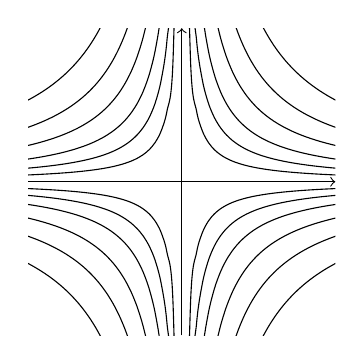
\begin{tikzpicture}[scale=0.75]
\begin{scope}
\clip (-2.6,-2.6) rectangle (2.6,2.6);
\foreach \c in {0.3,0.6,1,1.6,2.4,3.6}{
  \draw[domain=0.05:6,samples=60,smooth] plot(\x,{\c/\x});
  \draw[domain=0.05:6,samples=60,smooth] plot(-\x,{-\c/\x});
  \draw[domain=0.05:6,samples=60,smooth] plot(\x,{-\c/\x});
  \draw[domain=0.05:6,samples=60,smooth] plot(-\x,{\c/\x});
}
\end{scope}
\draw[->] (-2.6,0) -- (2.6,0);
\draw[->] (0,-2.6) -- (0,2.6);
\end{tikzpicture}
\end{center}

\vspace{4pt}
\noindent i. $f(x,y)=\dfrac{1}{x^2+y^2+1}$. \hspace{1cm} ii. $f(x,y)=xy$. \hspace{1cm} iii. $f(x,y)=x^2+y^2$. \hspace{1cm} iv. Ninguna de las anteriores.
\end{enumerate}

\newpage
\item{} (15\%) Hallar los puntos sobre el hiperboloide de una hoja $-x^2+z^2+y^2=1$ donde el plano tangente a él es paralelo al plano $z=4y-5$.

\vspace{8cm}

\item{} Sea $f:\mathbb{R}^2\to\mathbb{R}$ la función definida por
\[
f(x,y) = \left\{
\begin{array}{ll}
\dfrac{x^4+y^4}{x^2+y^2}+2x-y, & (x,y)\neq(0,0)\\[6pt]
0, & (x,y)=(0,0)
\end{array}
\right.
\]
\begin{enumerate}
\item{} (8\%) Encuentre $f_x(0,0)$ y $f_y(0,0)$.
\item{} (12\%) Muestre que $f$ es diferenciable en $(0,0)$.
\item{} (5\%) Encuentre la derivada direccional de $f$ en el punto $(0,0)$ en la dirección del vector $v=(3,-4)$.
\end{enumerate}

\vspace{8cm}

\newpage
\item{} (20\%) Sea $f:\mathbb{R}^2\to\mathbb{R}$ una función de clase $C^2$ de la cual se tiene la siguiente información:

\vspace{4pt}
\noindent $\nabla f(1,1)=(2,-3)$.

\noindent $\nabla f(0,1)=(5,-2)$.

\noindent $f_{xx}(1,1)=f_{yy}(1,1)=f_{xy}(1,1)=10$.

\noindent $f_{xx}(0,1)=f_{yy}(0,1)=f_{xy}(0,1)=-8$.

\vspace{4pt}
\noindent Definamos $g(u,v)=f(uv-1,2-u^2v)$.
\begin{enumerate}
\item{} (6\%) Encuentre una expresión para $g_u(u,v)$.
\item{} (14\%) Hallar $g_{uv}(1,1)$.
\end{enumerate}

\vspace{8cm}
\end{enumerate}

\examfooter
\end{document}
